\chapter{Test Problem}
\label{chap:testprob}

A simple test problem is described in this section.
Diagrams of the forward, adjoint, and contributon flux as well as the forward and adjoint current were produced to give insight into the physics of the test problem.
$\delta R\left(\vec{r}\right)$ was then calculated for several perturbations.

% The results were checked against MCNP results to verify that the method used to calculate $\delta R$ is correct.

%%%%%%%%%%%%%%%%%%%%%%%%%%%%%%%%%%%%%%%%%%%%%%%%%%%%%%%%%%%%%%%%%%%%%%%%%%%%%%%%
\section{Test Problem Overview}
\label{sec:bg:tp:overview}
%%%%%%%%%%%%%%%%%%%%%%%%%%%%%%%%%%%%%%%%%%%%%%%%%%%%%%%%%%%%%%%%%%%%%%%%%%%%%%%%

The test problem consists of an accelerator-based DD fusion neutron source (around 2.45 MeV), a tally region in which it is desired to maximize the ${}^{235}\text{U}$ fission rate, a moderating region, and an iron wall to separate the moderator from the tally region.
The goal of the test problem is to find the configuration of materials in the moderating region the produces the highest tally result.

The ``baseline'' moderator configuration is that it is entirely comprised of water.
All other configurations will be compared to the baseline.
A diagram of the baseline test problem geometry is shown in Figure \ref{fig:tp:material_map}.

\begin{figure}[h!]
  \centering
  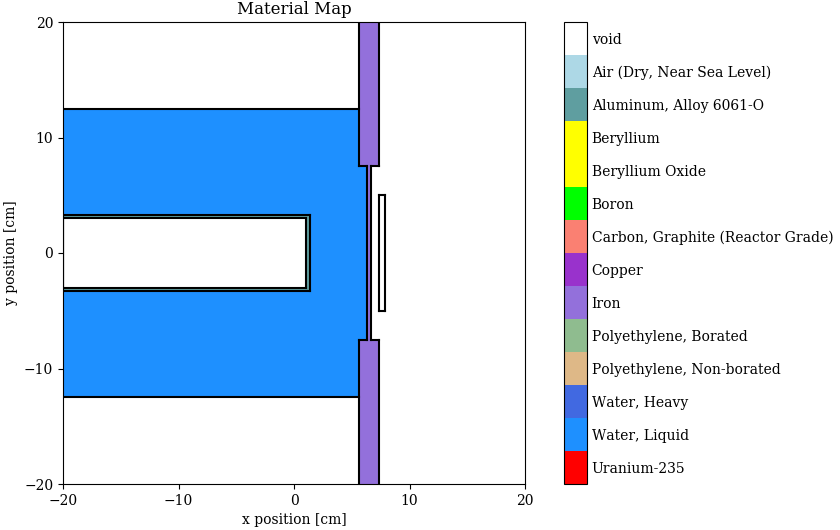
\includegraphics[width=0.75\linewidth]{content/testprob/material_map.png}
  \caption{Material map for test problem.}
  \label{fig:tp:material_map}
\end{figure}

The geometry is entirely comprised of rectangular parallelepipeds (RPPs in MCNP) to avoid there being mesh elements with mixed materials.
In ADVANTG, the 3D spatial mesh has 43 elements in the x-direction and 44 elements in both the y- and z-directions for a total of 83,248 voxels.

The ``27n19g'' multigroup cross section library, which contains 27 neutron energy groups and 19 gamma energy groups, was used.
Since the first neutron energy group in this library is above the maximum source energy, it is unused, leaving 26 neutron energy groups.
Since the tally is a neutron tally and the library does not account for photonuclear reactions, all of the gamma groups are also unused, leaving 26 total energy groups.
Upscattering was explicitly turned off for this analysis to decrease computation time.

The quadrupole range quadrature set with an order of 10 was used.
There were 4 azimuthal and 4 polar directions per octant, for a total of 16 directions per octant, or 128 directions overall.

The forward angular flux thus has $83,248 \times 26 \times 128 = 277,049,344$ values.
Even in this small test problem, the angular forward and adjoint fluxes combine to take up about 4.1 GB of storage space.

The locations of the energy-integrated source and response are shown in Figures \ref{fig:tp:source_total} and \ref{fig:tp:response_total}.
The source and response energy spectra are shown in \ref{fig:tp:spectra_lin}.
The source energy spectrum is spans the range between 1.97 and 3.23 MeV.
The response energy spectrum is equivalent to the ${}^{235}\text{U}$ fission cross section, which is highest at thermal energies.

\begin{figure}
  \centering
  \begin{minipage}{0.495\linewidth}
    \centering
    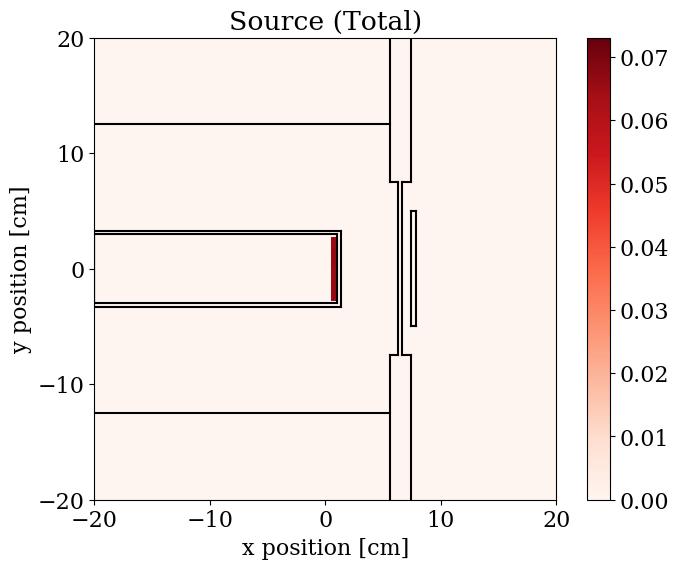
\includegraphics[width=\linewidth]{content/testprob/source_total.png}
    \caption{Location of energy-integrated source in test problem.}
    \label{fig:tp:source_total}
  \end{minipage}
  \hfill
  \begin{minipage}{0.495\linewidth}
    \centering
    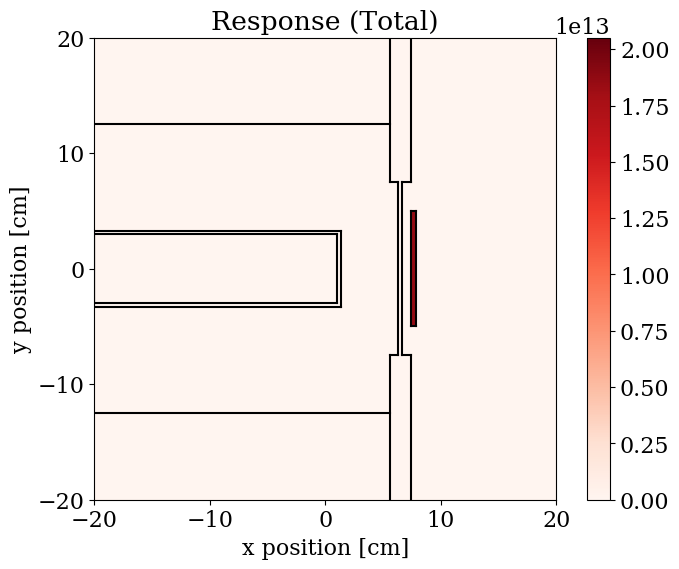
\includegraphics[width=\linewidth]{content/testprob/response_total.png}
    \caption{Location of energy-integrated response in test problem.}
    \label{fig:tp:response_total}
  \end{minipage}
  \centering
  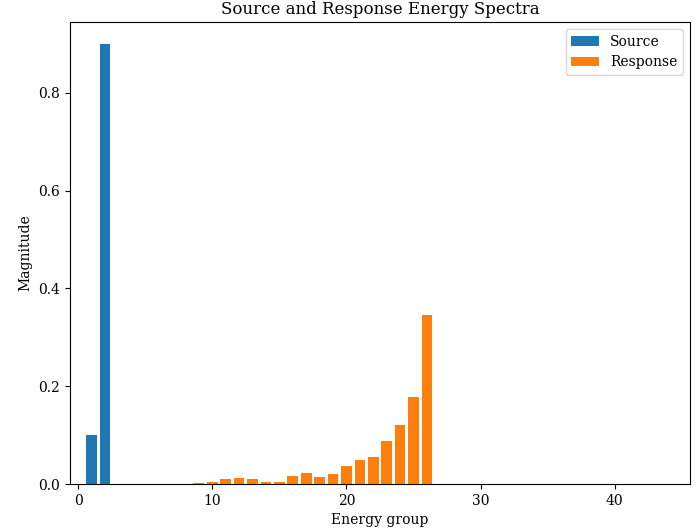
\includegraphics[width=0.6\linewidth]{content/testprob/spectra_lin.png}
  \caption{Source and response energy spectra in test problem.}
  \label{fig:tp:spectra_lin}
\end{figure}

%%%%%%%%%%%%%%%%%%%%%%%%%%%%%%%%%%%%%%%%%%%%%%%%%%%%%%%%%%%%%%%%%%%%%%%%%%%%%%%%
\section{Flux and Current in Test Problem}
\label{sec:bg:tp:flux}
%%%%%%%%%%%%%%%%%%%%%%%%%%%%%%%%%%%%%%%%%%%%%%%%%%%%%%%%%%%%%%%%%%%%%%%%%%%%%%%%

The scalar forward flux and forward current for energy group 2 (1.8268 to 3.0119 MeV) are shown in Figures \ref{fig:tp:scalar_flux_fwd_g02} and \ref{fig:tp:current_fwd_g02}.
The plots clearly show that fast neutron flux is highest close to the source, with fast neutrons radiating outward from that location.
Ray effects, which are caused by the angular discretization, are clearly visible in the plot of the scalar forward flux.

\begin{figure}
  \begin{minipage}{0.54\linewidth}
    \centering
    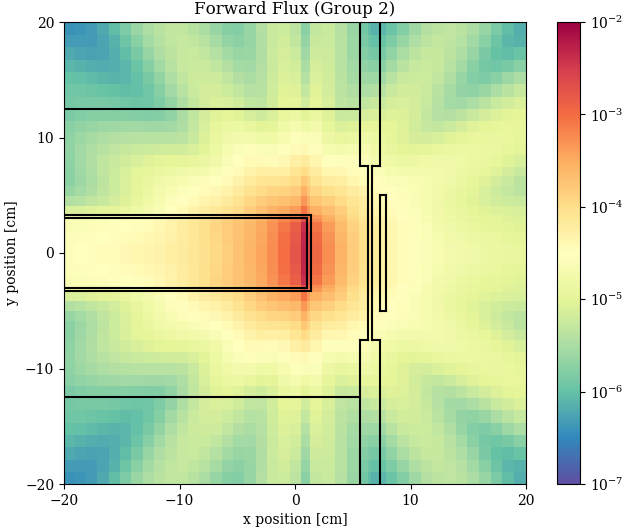
\includegraphics[width=\linewidth]{content/testprob/scalar_flux_fwd_g02.png}
    \caption{Scalar forward flux in energy group 2 in test problem.}
    \label{fig:tp:scalar_flux_fwd_g02}
  \end{minipage}
  \hfill
  \begin{minipage}{0.45\linewidth}
    \centering
    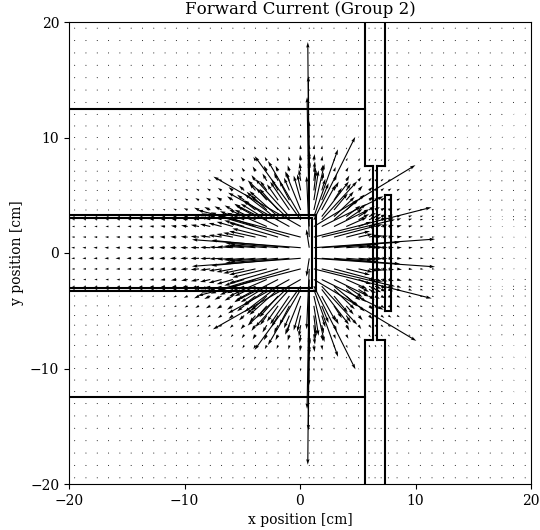
\includegraphics[width=\linewidth]{content/testprob/current_fwd_g02.png}
    \caption{Forward current in energy group 2 in test problem.}
    \label{fig:tp:current_fwd_g02}
  \end{minipage}
\end{figure}

The scalar forward flux and forward current for for energy group 25 ($10^{-8}$ to $3\times 10^{-8}$ MeV) are shown in Figures \ref{fig:tp:scalar_flux_fwd_g25} and \ref{fig:tp:current_fwd_g25}.
The plots show that the thermal neutron population is significantly mores spread out, existing as a cloud that encompasses most of the moderating region.
The thermal neutron flux is mostly isotropic within the moderating region.

\begin{figure}
  \begin{minipage}{0.54\linewidth}
    \centering
    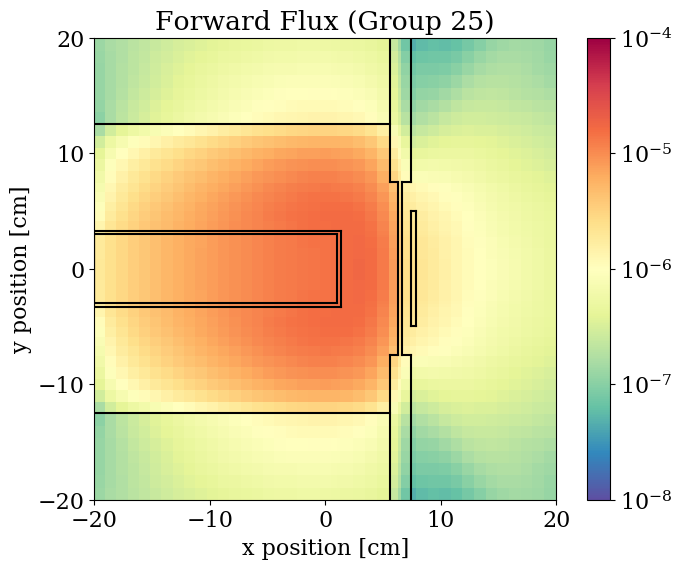
\includegraphics[width=\linewidth]{content/testprob/scalar_flux_fwd_g25.png}
    \caption{Scalar forward flux in energy group 25 in test problem.}
    \label{fig:tp:scalar_flux_fwd_g25}
  \end{minipage}
  \hfill
  \begin{minipage}{0.45\linewidth}
    \centering
    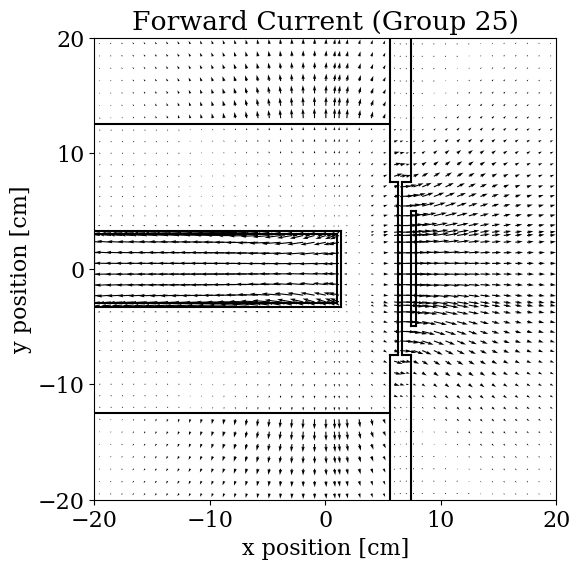
\includegraphics[width=\linewidth]{content/testprob/current_fwd_g25.png}
    \caption{Forward current in energy group 25 in test problem.}
    \label{fig:tp:current_fwd_g25}
  \end{minipage}
\end{figure}

The scalar adjoint flux and adjoint current for energy group 2 are shown in Figures \ref{fig:tp:scalar_flux_adj_g02} and \ref{fig:tp:current_adj_g02}.
The plots show that the region with the highest adjoint flux for fast neutrons is the region in between the source and detector, rather than at the detector itself.
This is an interesting result becuause it indicates that it is more likely that fast neutrons in the moderating region will thermalize and then contribute to the detector than it is that fast neutron already in the detector will contribute to it.
This effect is entirely due to the fact that ${}^{235}\text{U}$ has a fission cross section many orders of magnitude higher at thermal energies than it does at fast energies.

\begin{figure}
  \begin{minipage}{0.54\linewidth}
    \centering
    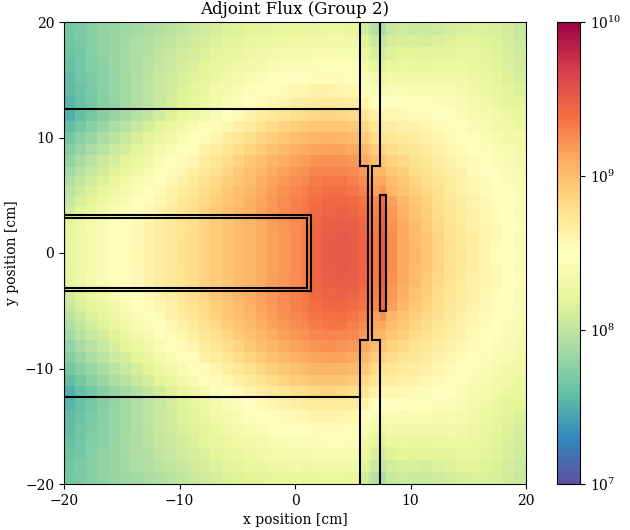
\includegraphics[width=\linewidth]{content/testprob/scalar_flux_adj_g02.png}
    \caption{Scalar adjoint flux in energy group 2 in test problem.}
    \label{fig:tp:scalar_flux_adj_g02}
  \end{minipage}
  \hfill
  \begin{minipage}{0.45\linewidth}
    \centering
    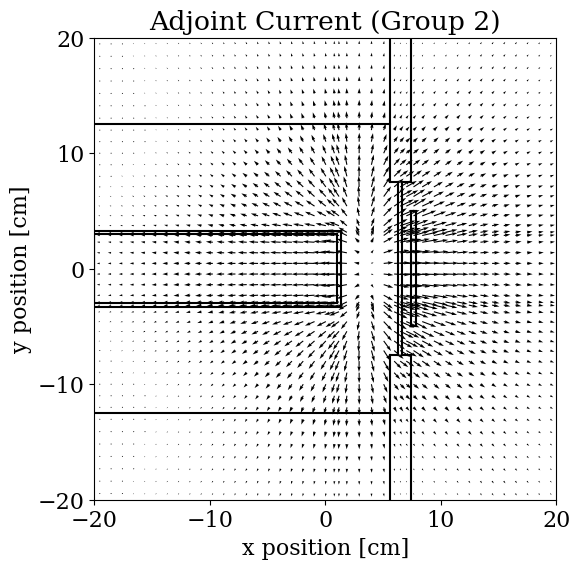
\includegraphics[width=\linewidth]{content/testprob/current_adj_g02.png}
    \caption{Adjoint current in energy group 2 in test problem.}
    \label{fig:tp:current_adj_g02}
  \end{minipage}
\end{figure}

The scalar adjoint flux and adjoint current for energy group 25 are shown in Figures \ref{fig:tp:scalar_flux_adj_g25} and \ref{fig:tp:current_adj_g25}.
The plots clearly show that the adjoint thermal flux radiates outward from the detector.
This means that the closer a thermal neutron is to the detector, the more likely it is to contribute.

\begin{figure}
  \begin{minipage}{0.54\linewidth}
    \centering
    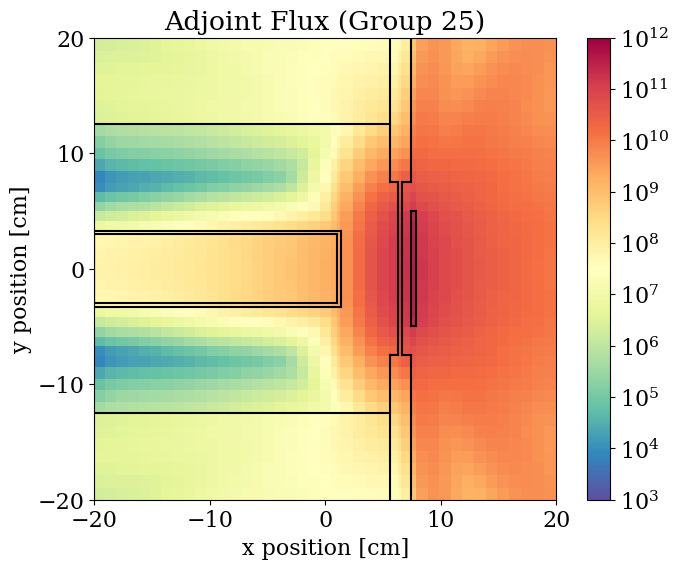
\includegraphics[width=\linewidth]{content/testprob/scalar_flux_adj_g25.png}
    \caption{Scalar adjoint flux in energy group 25 in test problem.}
    \label{fig:tp:scalar_flux_adj_g25}
  \end{minipage}
  \hfill
  \begin{minipage}{0.45\linewidth}
    \centering
    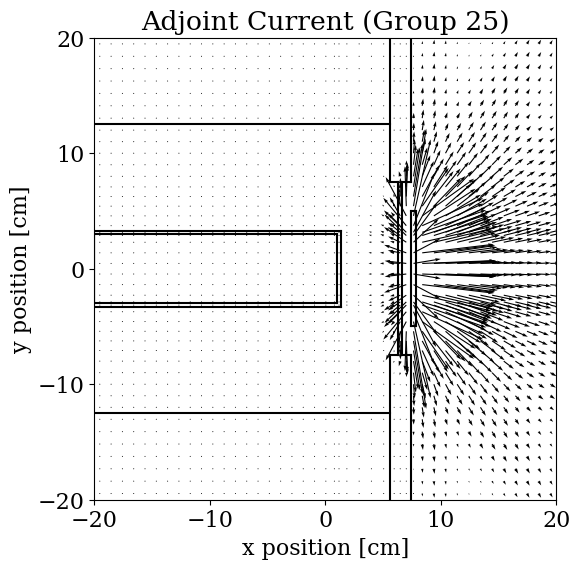
\includegraphics[width=\linewidth]{content/testprob/current_adj_g25.png}
    \caption{Adjoint current in energy group 25 in test problem.}
    \label{fig:tp:current_adj_g25}
  \end{minipage}
\end{figure}

The scalar contributon flux for energy groups 2 and 25 are shown in Figures \ref{fig:tp:scalar_flux_con_g02} and \ref{fig:tp:scalar_flux_con_g25}, and the scalar energy-integrated contributon flux is shown in Figure \ref{fig:tp:scalar_flux_con_total}.
Equation \ref{eq:bg:rt:scalar_contributon}, repeated here:
\begin{equation*}
  \Phi\left(\vec{r},E\right) \equiv
  \int_{4\pi}\psi\left(\vec{r},\hat{\Omega},E\right)\psi^+\left(\vec{r},-\hat{\Omega},E\right)d\hat{\Omega}.
\end{equation*}
defines the scalar contributon flux.
The contributon flux is at its highest in the region between the source and detector, which makes sense intuitively.
The physical interpretation of this result is that the region between the source and detector is the ``most important'' region of the problem.

Since the region on the right side of the problem is void, all forward and adjoint particles in that region are traveling to the right.
This is evident in Figures \ref{fig:tp:current_fwd_g02}, \ref{fig:tp:current_fwd_g25}, \ref{fig:tp:current_adj_g02}, and \ref{fig:tp:current_adj_g25}: all current vectors in the void region on the right side of the problem are aiming to the right in some manner; none are aiming left.
Thus, after noting that the directionality of the adjoint flux is reversed in the equation for the contributon flux, the contributon flux in that region is zero.

\begin{figure}
  \begin{minipage}{0.495\linewidth}
    \centering
    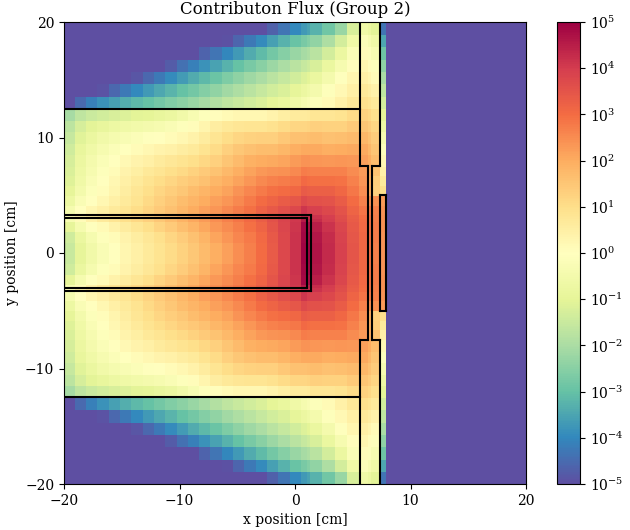
\includegraphics[width=\linewidth]{content/testprob/scalar_flux_con_g02.png}
    \caption{Contributon flux in energy group 2 in test problem.}
    \label{fig:tp:scalar_flux_con_g02}
  \end{minipage}
  \hfill
  \begin{minipage}{0.495\linewidth}
    \centering
    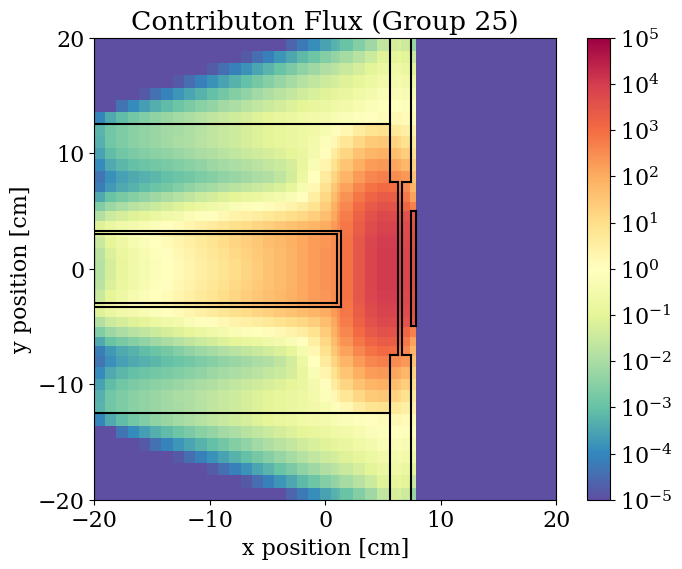
\includegraphics[width=\linewidth]{content/testprob/scalar_flux_con_g25.png}
    \caption{Contributon flux in energy group 25 in test problem.}
    \label{fig:tp:scalar_flux_con_g25}
  \end{minipage}
  \centering
  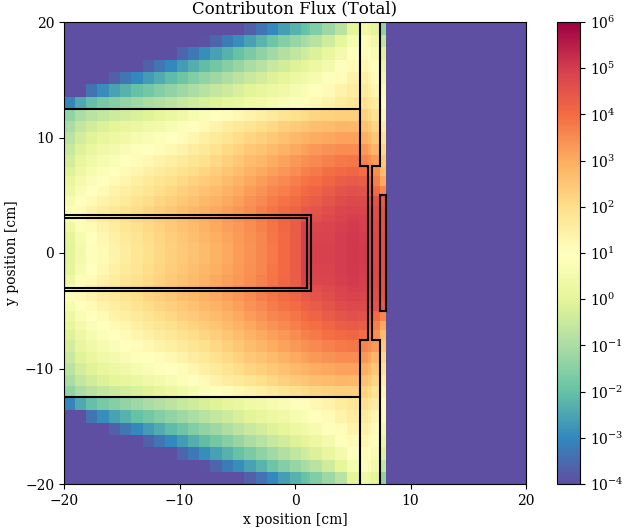
\includegraphics[width=0.495\linewidth]{content/testprob/scalar_flux_con_total.png}
  \caption{Energy-integrated contributon flux in test problem.}
  \label{fig:tp:scalar_flux_con_total}
\end{figure}

%%%%%%%%%%%%%%%%%%%%%%%%%%%%%%%%%%%%%%%%%%%%%%%%%%%%%%%%%%%%%%%%%%%%%%%%%%%%%%%%
\section{Calculation of $\delta R$ in Test Problem}
\label{sec:bg:tp:dr}
%%%%%%%%%%%%%%%%%%%%%%%%%%%%%%%%%%%%%%%%%%%%%%%%%%%%%%%%%%%%%%%%%%%%%%%%%%%%%%%%

Equation \ref{eq:dr:dr_function_of_position_final}, repeated here:
\begin{multline*}
  \delta R\left(\vec{r}\right) =
  \int_0^\infty\phi^+\left(\vec{r},E\right)\left(\int_0^\infty\delta\sigma_s\left(\vec{r},E^\prime\rightarrow E\right)\phi\left(\vec{r},E^\prime\right)dE^\prime\right)dE - \\
  \int_0^\infty\delta\sigma_t\left(\vec{r},E\right)\Phi\left(\vec{r},E\right)dE,
\end{multline*}
was used to calculate $\delta R$ in the test problem.
The value of $\delta R$ at point $\vec{r}_0$; i.e. $\delta R\left(\vec{r}_0\right)$, refers to the perturbation in the detector response given a perturbation in the cross sections ($\delta \sigma_t$ and $\delta \sigma_s$) that only occurs at point $\vec{r}_0$.
The vector quantity $\delta R\left(\vec{r}\right)$ is constructed by calculating $\delta R\left(\vec{r}_0\right)$ for the entire problem domain.

In the test problem, the perturbation at point $\vec{r}_0$ was defined as the difference in cross sections between some new material and the existing material at point $\vec{r}_0$.
$\delta R\left(\vec{r}\right)$ was only calculated for $\vec{r}$ inside the moderating region, as this is the region of interest.

$\delta R\left(\vec{r}\right)$ was calculated for several different materials, which are listed in Table \ref{tab:testprob:material_list}.
The materials are separated into several categories:
\begin{enumerate}
  \item Low-density: these materials have low or zero density, and are expected to perform poorly as replacement moderators.
  \item Moderating:  these materials are all used as moderators in real-world nuclear systems, so they are expected to perform the best of all materials.
  \item Structural:  these materials are commonly used for structural purposes and are not good moderators, so they are expected to perform poorly.
  \item Absorbing:   these materials are known absorbers of thermal neutrons, so they are expected to perform the the worst.
% \item Fissile:     these materials are neutron multipliers, which means they should perform well in theory, but since the cross section libraries available in ADVANTG do not take fission into account, the results are expected to be poor.
\end{enumerate}

\begin{table}[h]
  \centering
  \caption{List of materials considered in the test problem.}
  \label{tab:testprob:material_list}
  \begin{tabular}{| c | c | c |}
    \hline
    \textbf{Material}     & \textbf{Group}       \\ \hline
    Void                  & Low-density          \\ \hline  %  0
    Air                   & Low-density          \\ \hline  %  1
%   Beryllium             & Moderating           \\ \hline  %  3
    Beryllium oxide (BeO) & Moderating           \\ \hline  %  4
    Graphite              & Moderating           \\ \hline  %  6
    Water                 & Moderating           \\ \hline  % 14
    Heavy water           & Moderating           \\ \hline  % 13
    HDPE                  & Moderating           \\ \hline  % 12
    Borated HDPE          & Moderating/absorbing \\ \hline  % 11
    Concrete              & Structural           \\ \hline  %  7
    Aluminum              & Structural           \\ \hline  %  2
    Iron                  & Structural           \\ \hline  % 10
    Copper                & Structural           \\ \hline  %  8
%   Ziracloy-4            & Structural           \\ \hline  % 15
    Boron                 & Absorbing            \\ \hline  %  5
    Gadolinium            & Absorbing            \\ \hline  %  9
%   ${}^{235}\text{U}$    & Fissile              \\ \hline  % 16
  \end{tabular}
\end{table}

In all plots of $\delta R\left(\vec{r}\right)$, positive values are shown in red and negative values are shown in blue.
A positive values of $\delta R\left(\vec{r}_0\right)$ indicates that replacing the existing material only at point $\vec{r}_0$ with the new material results in an increase in the detector response.
A negative value indicates that replacing the material at point $\vec{r}_0$ results in a decrease in the detector response.
If the existing material and the new material at a point are the same, then the value of $\delta R$ at that point will be zero.

Plots of $\delta R$ for the low-density materials are shown in Figures \ref{fig:tp:dR_00} and \ref{fig:tp:dR_01}.
These plots show that replacing any part of the moderating region with void or air results in a decrease in the detector response.
This is an expected result.
The existing moderator serves an important purpose: it acts to thermalize the neutrons so they have lower energy when reaching the detector, which leads to an increase in the detector response because the detector responds much more strongly to thermal neutrons.
Thus, it makes sense that removing any part of the moderator would decrease the amount of thermalization taking place, which in turn would decrease the detector response.

\begin{figure}
  \begin{minipage}{0.495\linewidth}
    \centering
    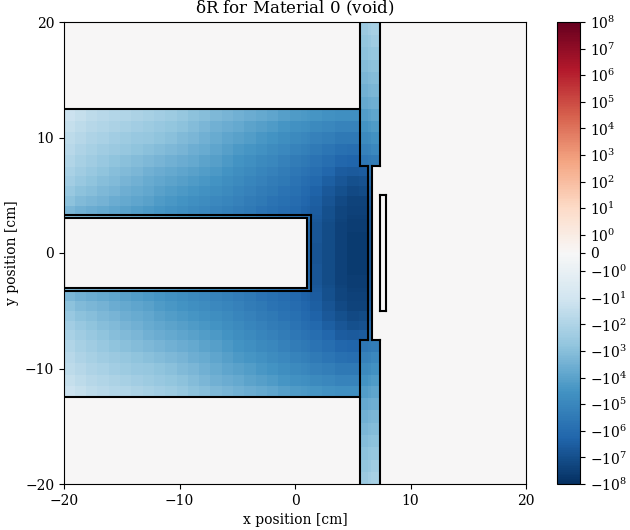
\includegraphics[width=\linewidth]{content/testprob/dR_00.png}
    \caption{$\delta R$ for void in test problem.}
    \label{fig:tp:dR_00}
  \end{minipage}
  \hfill
  \begin{minipage}{0.495\linewidth}
    \centering
    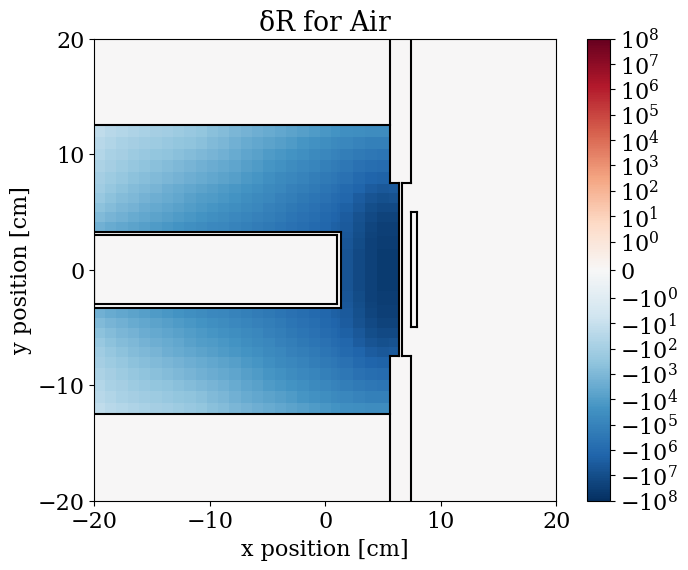
\includegraphics[width=\linewidth]{content/testprob/dR_01.png}
    \caption{$\delta R$ for air in test problem.}
    \label{fig:tp:dR_01}
  \end{minipage}
\end{figure}

Plots of $\delta R$ for some common moderating materials are shown in Figures \ref{fig:tp:dR_04}, \ref{fig:tp:dR_06}, \ref{fig:tp:dR_14}, \ref{fig:tp:dR_13}, \ref{fig:tp:dR_12}, and \ref{fig:tp:dR_11}.
The plots show that replacing any part of the existing water moderator water with graphite or heavy water would result in a decrease in the detector response.
This is likely due to the fact that the mean number of collisions to achieve thermalization is higher in graphite and heavy water than it is in water.

It is also apparent that replacing any part of the existing water moderator with HDPE or borated HDPE would result in an increase in the detector response.
The result for HDPE makes sense because HDPE has a higher hydrogen density than water which leads to similar amounts of thermalization occurring over less distance.
The result for borated HDPE does not make much sense, however, because boron is a known strong absorber of thermal neutrons, and boron should serve to reduce the thermal neutron population.
More analysis is needed to understand the result for borated HDPE.

BeO is an interesting case: in the region between the source and detector, it performs worse than water, while in the region behind the source, it performs better.
This result shows that the optimal moderator configuration likely includes two or more materials.

The plot for water is shown simply as a sanity check.
Since the existing moderator is already comprised of water, the detector response does not change when water is replaced with itself.

\begin{figure}
  \begin{minipage}{0.495\linewidth}
    \centering
    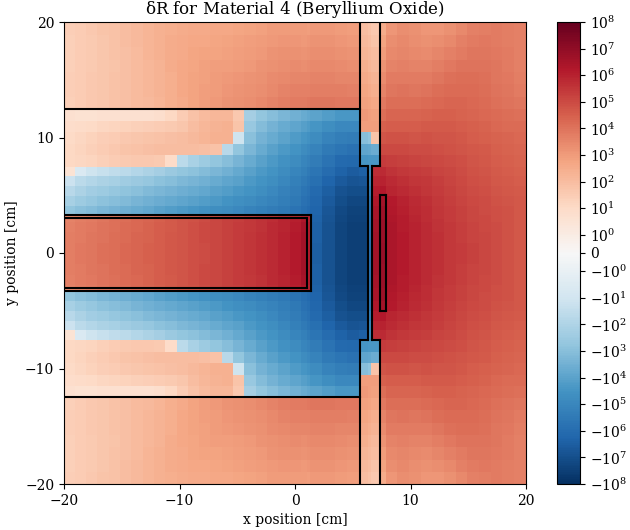
\includegraphics[width=\linewidth]{content/testprob/dR_04.png}
    \caption{$\delta R$ for beryllium oxide (BeO) in test problem.}
    \label{fig:tp:dR_04}
  \end{minipage}
  \hfill
  \begin{minipage}{0.495\linewidth}
    \centering
    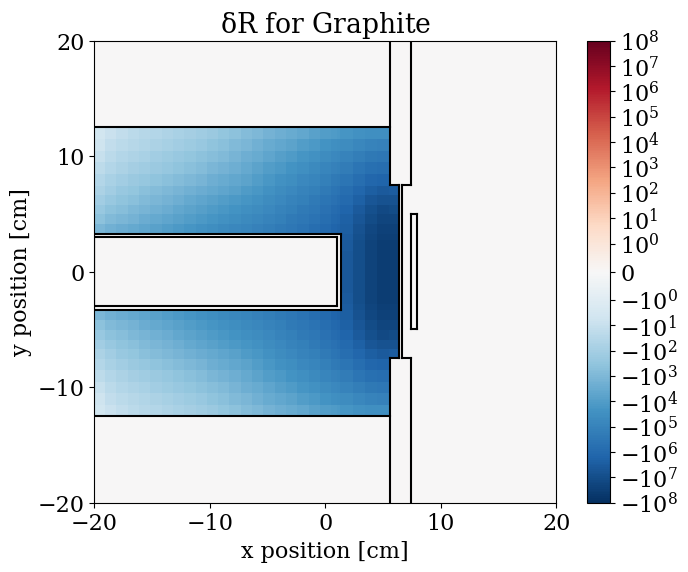
\includegraphics[width=\linewidth]{content/testprob/dR_06.png}
    \caption{$\delta R$ for graphite in test problem.}
    \label{fig:tp:dR_06}
  \end{minipage}
  \begin{minipage}{0.495\linewidth}
    \centering
    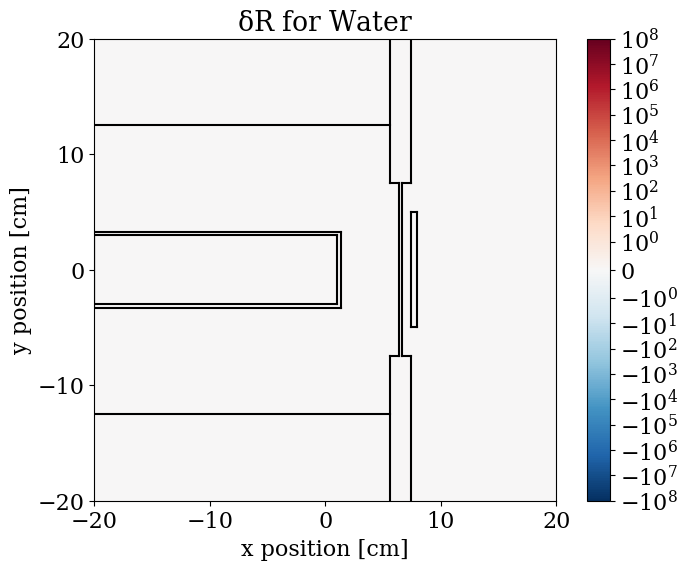
\includegraphics[width=\linewidth]{content/testprob/dR_14.png}
    \caption{$\delta R$ for water in test problem.}
    \label{fig:tp:dR_14}
  \end{minipage}
  \hfill
  \begin{minipage}{0.495\linewidth}
    \centering
    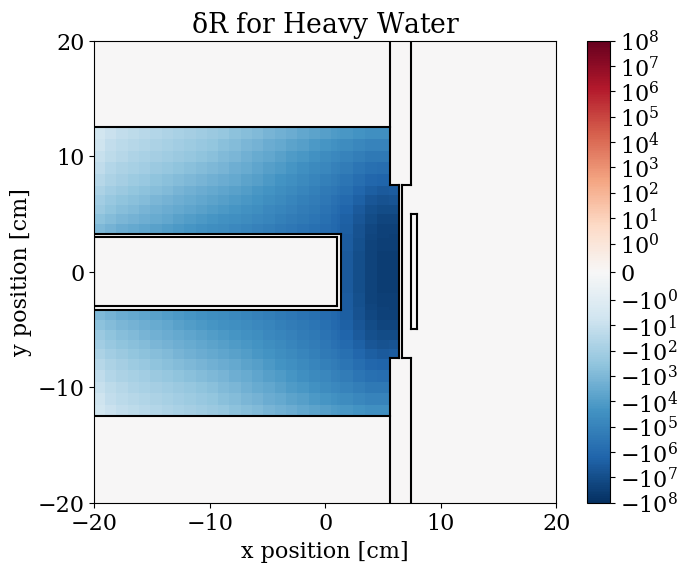
\includegraphics[width=\linewidth]{content/testprob/dR_13.png}
    \caption{$\delta R$ for heavy water in test problem.}
    \label{fig:tp:dR_13}
  \end{minipage}
  \begin{minipage}{0.495\linewidth}
    \centering
    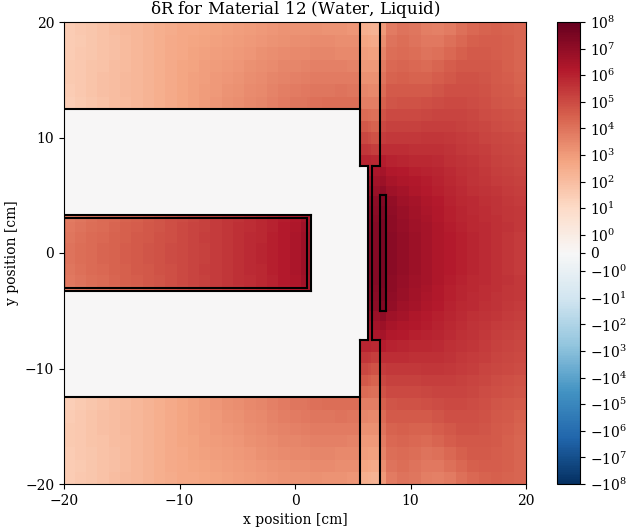
\includegraphics[width=\linewidth]{content/testprob/dR_12.png}
    \caption{$\delta R$ for HDPE in test problem.}
    \label{fig:tp:dR_12}
  \end{minipage}
  \hfill
  \begin{minipage}{0.495\linewidth}
    \centering
    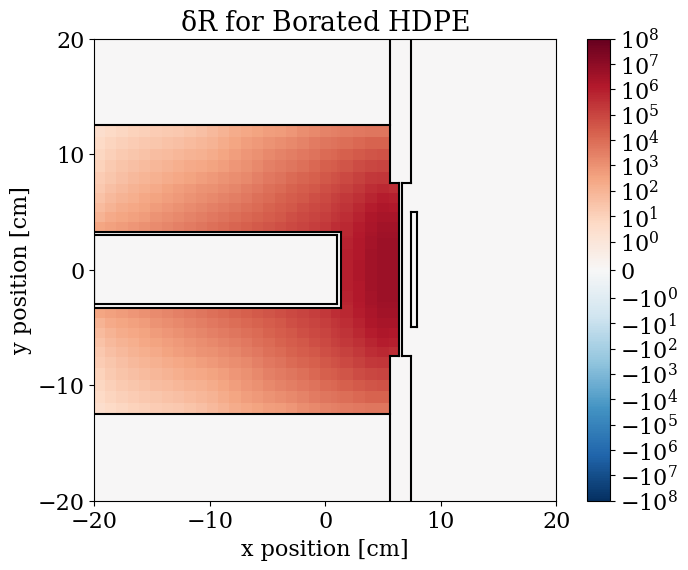
\includegraphics[width=\linewidth]{content/testprob/dR_11.png}
    \caption{$\delta R$ for borated HDPE in test problem.}
    \label{fig:tp:dR_11}
  \end{minipage}
\end{figure}

Plots of $\delta R$ for some common structural materials are shown in Figures \ref{fig:tp:dR_07}, \ref{fig:tp:dR_02}, \ref{fig:tp:dR_10}, and \ref{fig:tp:dR_08}.
The plots show that all four materials perform considerably worse than water at every location in the moderator.
This was expected because none of these materials are considered to be effective moderators.

\begin{figure}
  \begin{minipage}{0.495\linewidth}
    \centering
    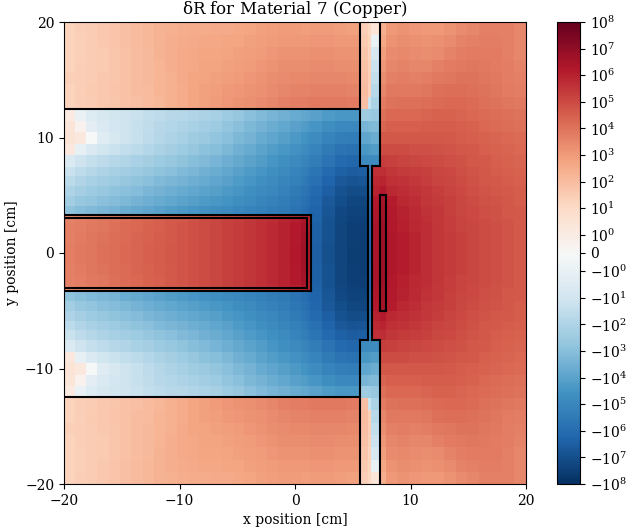
\includegraphics[width=\linewidth]{content/testprob/dR_07.png}
    \caption{$\delta R$ for concrete in test problem.}
    \label{fig:tp:dR_07}
  \end{minipage}
  \hfill
  \begin{minipage}{0.495\linewidth}
    \centering
    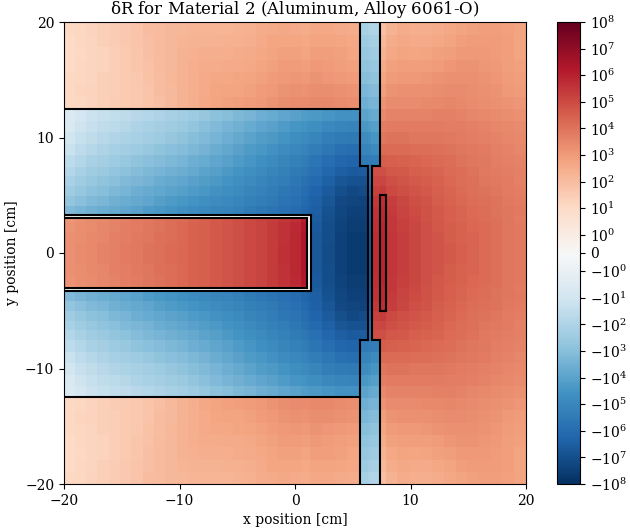
\includegraphics[width=\linewidth]{content/testprob/dR_02.png}
    \caption{$\delta R$ for aluminum in test problem.}
    \label{fig:tp:dR_02}
  \end{minipage}
  \begin{minipage}{0.495\linewidth}
    \centering
    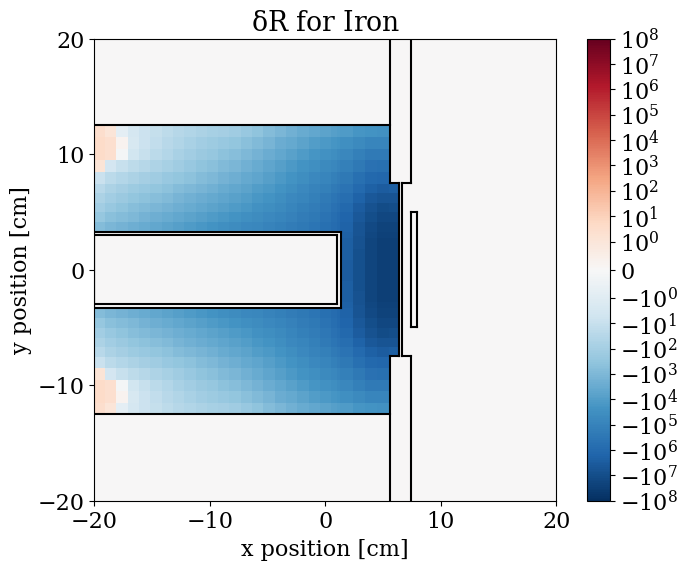
\includegraphics[width=\linewidth]{content/testprob/dR_10.png}
    \caption{$\delta R$ for iron in test problem.}
    \label{fig:tp:dR_10}
  \end{minipage}
  \hfill
  \begin{minipage}{0.495\linewidth}
    \centering
    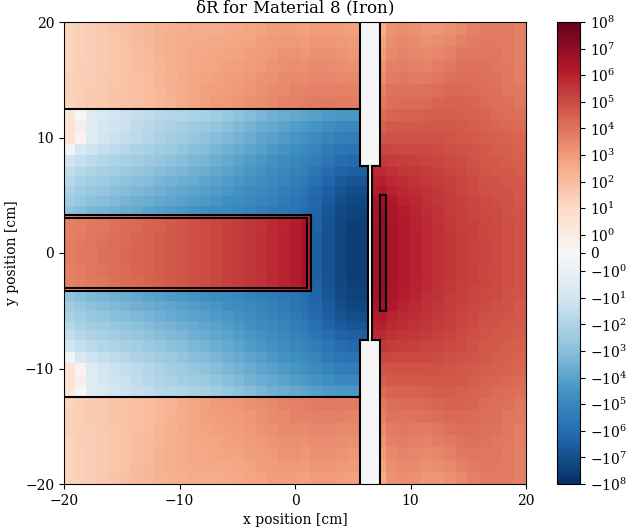
\includegraphics[width=\linewidth]{content/testprob/dR_08.png}
    \caption{$\delta R$ for copper in test problem.}
    \label{fig:tp:dR_08}
  \end{minipage}
\end{figure}

Plots of $\delta R$ for some thermal neutron absorbers are shown in Figures \ref{fig:tp:dR_05} and \ref{fig:tp:dR_09}.
These materials performed even worse than the structural materials, which was expected because of their large absorption cross sections at thermal energies.

\begin{figure}
  \begin{minipage}{0.495\linewidth}
    \centering
    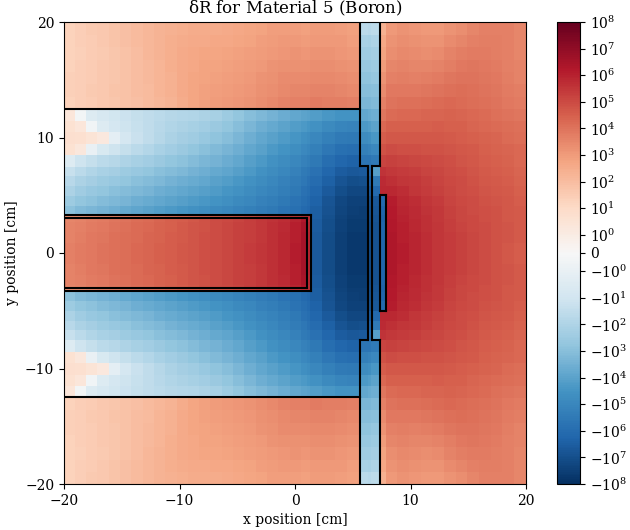
\includegraphics[width=\linewidth]{content/testprob/dR_05.png}
    \caption{$\delta R$ for boron in test problem.}
    \label{fig:tp:dR_05}
  \end{minipage}
  \hfill
  \begin{minipage}{0.495\linewidth}
    \centering
    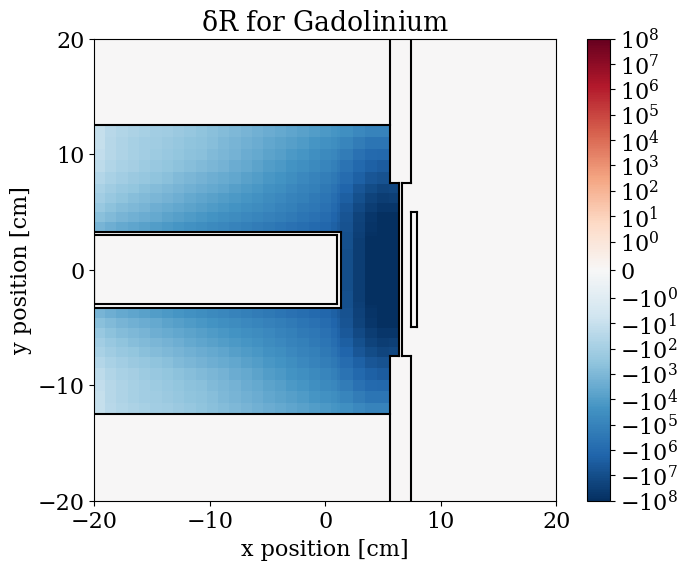
\includegraphics[width=\linewidth]{content/testprob/dR_09.png}
    \caption{$\delta R$ for gadolinium in test problem.}
    \label{fig:tp:dR_09}
  \end{minipage}
\end{figure}

% %%%%%%%%%%%%%%%%%%%%%%%%%%%%%%%%%%%%%%%%%%%%%%%%%%%%%%%%%%%%%%%%%%%%%%%%%%%%%%%%
% \section{MCNP Validation}
% \label{sec:bg:tp:mcnp}
% %%%%%%%%%%%%%%%%%%%%%%%%%%%%%%%%%%%%%%%%%%%%%%%%%%%%%%%%%%%%%%%%%%%%%%%%%%%%%%%%
